%%%%%%%%%%%%%%%%%%%%%%%%%%%%%%%%%%%%%%%%%
% Journal Article
% LaTeX Template
% Version 1.4 (15/5/16)
%
% This template has been downloaded from:
% http://www.LaTeXTemplates.com
%
% Original author:
% Frits Wenneker (http://www.howtotex.com) with extensive modifications by
% Vel (vel@LaTeXTemplates.com)
%
% License:
% CC BY-NC-SA 3.0 (http://creativecommons.org/licenses/by-nc-sa/3.0/)
%
%%%%%%%%%%%%%%%%%%%%%%%%%%%%%%%%%%%%%%%%%

%----------------------------------------------------------------------------------------
%	PACKAGES AND OTHER DOCUMENT CONFIGURATIONS
%----------------------------------------------------------------------------------------

\documentclass[twoside,onecolumn]{article}

\usepackage{blindtext} % Package to generate dummy text throughout this template 
\usepackage{graphicx}
\graphicspath{ {Imagenes/} }
\usepackage[sc]{mathpazo} % Use the Palatino font
\usepackage[T1]{fontenc} % Use 8-bit encoding that has 256 glyphs
\linespread{1.05} % Line spacing - Palatino needs more space between lines
\usepackage{microtype} % Slightly tweak font spacing for aesthetics

\usepackage[english]{babel} % Language hyphenation and typographical rules

\usepackage[hmarginratio=1:1,top=32mm,columnsep=20pt]{geometry} % Document margins
\usepackage[hang, small,labelfont=bf,up,textfont=it,up]{caption} % Custom captions under/above floats in tables or figures
\usepackage{booktabs} % Horizontal rules in tables

\usepackage{lettrine} % The lettrine is the first enlarged letter at the beginning of the text

\usepackage{enumitem} % Customized lists
\setlist[itemize]{noitemsep} % Make itemize lists more compact

\usepackage{abstract} % Allows abstract customization
\renewcommand{\abstractnamefont}{\normalfont\bfseries} % Set the "Resumen" text to bold
\renewcommand{\abstracttextfont}{\normalfont\small\itshape} % Set the abstract itself to small italic text

\usepackage{titlesec} % Allows customization of titles
\renewcommand\thesection{\Roman{section}} % Roman numerals for the sections
\renewcommand\thesubsection{\roman{subsection}} % roman numerals for subsections
\titleformat{\section}[block]{\large\scshape\centering}{\thesection.}{1em}{} % Change the look of the section titles
\titleformat{\subsection}[block]{\large}{\thesubsection.}{0.2em}{} % Change the look of the section titles

\usepackage{fancyhdr} % Headers and footers
\pagestyle{fancy} % All pages have headers and footers
\fancyhead{} % Blank out the default header
\fancyfoot{} % Blank out the default footer
\fancyhead[C]{Comparación de despliegue de un gestor de base de datos NoSQL mediante Docke $\bullet$ Junio 2019 $\bullet$ Trabajo Final} % Custom header text
\fancyfoot[RO,LE]{\thepage} % Custom footer text

\usepackage{titling} % Customizing the title section

\usepackage{hyperref} % For hyperlinks in the PDF

%----------------------------------------------------------------------------------------
%	TITLE SECTION
%----------------------------------------------------------------------------------------
\setlength{\droptitle}{-4\baselineskip} % Move the title up

\pretitle{\begin{center}\Huge\bfseries} % Article title formatting
\posttitle{\end{center}} % Article title closing formatting
\title{Comparación de Despliegue de un Gestor de Base de Datos NoSQL Mediante Docker} % Article title
\author{%
\textsc{Marko Antonio Rivas Rios} \\[1ex] % Your name
\textsc{Jorge Luis Mamani Maquera} \\[1.01ex] % Your name
\textsc{Orlando Antonio Acosta Ortiz} \\[1.02ex] % Your name
\textsc{Yofer Nain Catari Cabrera} \\[1.03ex] % Your name
\textsc{Orestes Ramirez Ticona} \\[1.04ex] % Your name
\textsc{Roberto Zegarra Reyes} \\[1.05ex] % Your name
\normalsize Universidad Privada de Tacna \\  % Your institution
\normalsize {} % Your email address
%\and % Uncomment if 2 authors are required, duplicate these 4 lines if more
%\textsc{Jane Smith}\thanks{Corresponding author} \\[1ex] % Second author's name
%\normalsize University of Utah \\ % Second author's institution
%\normalsize \href{mailto:jane@smith.com}{jane@smith.com} % Second author's email address
}
\date{Junio 22, 2019} % Leave empty to omit a date
\renewcommand{\maketitlehookd}{%
\begin{abstract}
\begin{center}
\textbf{Resumen}
\end{center}
\noindent Docker es un proyecto open source creado en 2013 y que ha supuesto una revolución para el desarrollo y despliegue de operaciones. Docker abstrae el hardware y el sistema operativo del host ejecutando las aplicaciones en contenedores, compartimentos aislados que contienen todos los recursos para una aplicación o servicio. En este trabajo veremos cómo usar Docker para el desarrollo de aplicaciones sencillas, aprendiendo a desplegar una base de datos NOSQL con Docker.
\begin{center}
\textbf{Abstract}
\end{center}
\noindent Docker is an open source project created in 2013 and which has been a revolution for the development and deployment of operations. Docker abstracts the host's hardware and operating system by running the applications in containers, isolated compartments that contain all the resources for an application or service.
In this work we will see how to use Docker for the development of simple applications, learning how to deploy a NOSQL database with Docker.
\end{abstract}
}


%----------------------------------------------------------------------------------------

\begin{document}

% Print the title
\maketitle

%----------------------------------------------------------------------------------------
%	ARTICLE CONTENTS
%----------------------------------------------------------------------------------------

\section{Introducción}

\lettrine[nindent=0em,lines=2]{E}l potente concepto de Microservicios está cambiando poco a poco la industria. Grandes servicios monolíticos están dando paso lentamente al enjambre microservicios pequeños y autónomos que trabajan en conjunto. El proceso va acompañado de otra tendencia del mercado: la contenerización. Juntos, ayudan a construir sistemas  sin precedentes. La contenerización cambia no sólo la arquitectura de los servicios, sino también la estructura de ambientes utilizados para crearlos.
\textbf{}\\
Ahora, cuando el software se distribuye en contenedores, los desarrolladores tienen plena libertad para decidir qué aplicaciones necesitan. Como resultado, incluso los entornos complejos, como los servidores de grades bases de datos e infraestructura de análisis complejos pueden crear instancias en cuestión de segundos. El desarrollo de software se hace más fácil y más eficaz.

\section{Materiales y Métodos}
\subsection{Materiales}
	\begin{itemize}
		\item Virtualización activada en el BIOS
		\item Docker Desktop
		\item Windows 10 64bit: Pro, Enterprise o Education, con al menos 4GB de RAM.
	\end{itemize}
\subsection{Métodos}
	\begin{itemize}
		\item Se utilizo como material artículos y libros relacionados a la base de datos NoSQL y sus tipos, así como páginas web.
	\end{itemize}
\begin{flushright}
\begin{itemize}
%------------------------------------------------

\section{Marco Teórico}

Docker es una tecnología de containers muy popular.
¿No has usado containers? Sirven para desplegar aplicaciones en un entorno virtual aislado, pero sin el overhead de tener un Sistema Operativo (SO) nuevo como se tiene en una Virtual Machine (VM).\textbf{}\\
La principal diferencia es que los containers virtualizan el SO en vez del hardware, como lo hace una VM. De esta forma un container usa menos espacio en disco (ya que no requiere una copia del SO), y es más ágil (ya que usa menos recursos del host para ejecutar).

\textbf{}\\
\subsection{Creación de una base de datos NoSQL en docker}
\textbf{}\\
Instala Docker Desktop para Windows
Docker Desktop para Windows es la Community Edition (CE) de Docker para Microsoft Windows. Para descargar Docker Desktop para Windows, diríjase a Docker Hub.
\textbf{}\\
\textbf{}\\
Lo que hay que saber antes de instalar es: \textbf{}\\
README FIRST para los usuarios de Docker Toolbox y Docker Machine : Docker Desktop para Windows requiere Microsoft Hyper-V para ejecutarse. El instalador de Docker Desktop para Windows habilita Hyper-V para usted, si es necesario, y reinicia su máquina. Después de habilitar Hyper-V, VirtualBox ya no funciona, pero las imágenes de VirtualBox VM permanecen. Las máquinas virtuales de VirtualBox creadas con docker-machine(incluida la defaultque se crea normalmente durante la instalación de Toolbox) ya no se inician. Estas máquinas virtuales no se pueden usar en paralelo con Docker Desktop para Windows. Sin embargo, todavía puede utilizar docker-machinepara administrar máquinas virtuales remotas.
\textbf{}\\
\textbf{}\\
\textbf{Requisitos del sistema :}\\
- Windows 10 64bit: Pro, Enterprise o Education (Build 15063 o posterior).\textbf{}\\
- La virtualización está habilitada en la BIOS. Normalmente, la virtualización está habilitada por defecto. Esto es diferente de tener Hyper-V habilitado. Para obtener más detalles, consulte La virtualización debe estar habilitada en Solución de problemas.\textbf{}\\
- Característica capaz de CPU SLAT.\textbf{}\\
- Al menos 4GB de RAM.\textbf{}\\
\textbf{}\\
\textbf{}\\
Nota : Si su sistema no cumple con los requisitos para ejecutar Docker Desktop para Windows, puede instalar Docker Toolbox , que utiliza Oracle Virtual Box en lugar de Hyper-V.
\textbf{}\\
\textbf{}\\

Lo que incluye la instalación de Docker Desktop para Windows : La instalación proporciona Docker Engine , Docker CLI client, Docker Compose , Docker Machine y Kitematic .
Los contenedores y las imágenes creadas con Docker Desktop para Windows se comparten entre todas las cuentas de usuario en las máquinas donde está instalado. Esto se debe a que todas las cuentas de Windows usan la misma máquina virtual para crear y ejecutar contenedores.\textbf{}\\
Los escenarios de virtualización anidados, como ejecutar Docker Desktop para Windows en una instancia de VMWare o Parallels, pueden funcionar, pero no hay garantías. Para obtener más información, consulte Ejecución de Docker Desktop para Windows en escenarios de virtualización anidados.\textbf{}\\
\textbf{}\\
Instalar la aplicación de escritorio Docker Desktop para Windows
\textbf{}\\
1.- Haga doble clic en Docker Desktop para Windows Installer.exe para ejecutar el instalador.
Si aún no ha descargado el instalador ( Docker Desktop Installer.exe), puede obtenerlo en download.docker.com . Normalmente se descarga a su Downloadscarpeta, o puede ejecutarlo desde la barra de descargas recientes en la parte inferior de su navegador web.
\textbf{}\\
\textbf{}\\
2.-Siga el asistente de instalación para aceptar la licencia, autorice el instalador y continúe con la instalación.
Se le solicitará que autorice Docker.appcon su contraseña del sistema durante el proceso de instalación. Se necesita acceso privilegiado para instalar componentes de red, enlaces a las aplicaciones de Docker y administrar las máquinas virtuales de Hyper-V.
\textbf{}\\
\textbf{}\\
3.-Haga clic en Finalizar en el cuadro de diálogo de instalación completa para iniciar Docker.

\textbf{}\\
Iniciar Docker Desktop para Windows
\textbf{}\\
Docker no se inicia automáticamente después de la instalación. Para iniciarlo, busque Docker, seleccione Docker Desktop para Windows en los resultados de búsqueda y haga clic en él (o presione Entrar).
\textbf{}\\
\begin{center}
		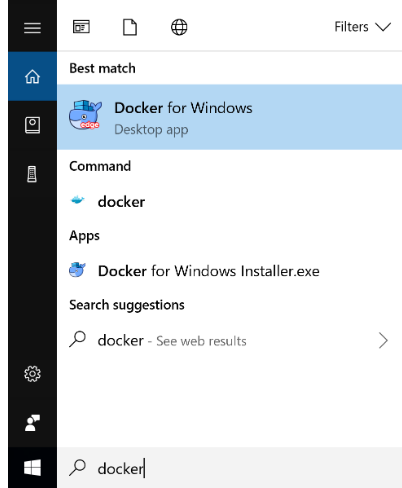
\includegraphics[width=9cm]{./Imagenes/n1.png}
\end{center}	
\textbf{}\\
Cuando la ballena en la barra de estado se mantiene estable, Docker está en funcionamiento y accesible desde cualquier ventana de terminal.
\begin{center}
		
\includegraphics[width=9cm]{./Imagenes/n2.png}
\end{center}	
\textbf{}\\
Si la ballena está oculta en el área de Notificaciones, haga clic en la flecha hacia arriba en la barra de tareas para mostrarla. Para obtener más información, consulte Configuración de Docker .
Si acaba de instalar la aplicación, también recibe un mensaje emergente de éxito con los siguientes pasos sugeridos y un enlace a esta documentación.
\textbf{}\\
\begin{center}
		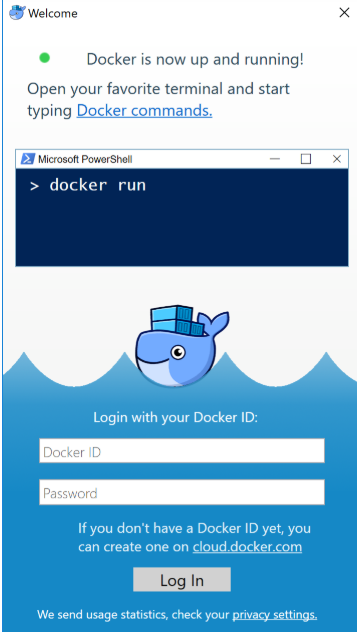
\includegraphics[width=9cm]{./Imagenes/n3.png}
\end{center}	
Cuando se complete la inicialización, seleccione Acerca de Docker en el ícono del área de Notificaciones para verificar que tiene la última versión.
Está en funcionamiento con Docker Desktop para Windows.
\textbf{}\\

\textbf{Creacion de base de datos NoSQL con MongoDB en Docker}\\

\textbf{}\\
\textbf{Instalar MongoDB en Docker}\\
\textbf{}\\
- Ingresar sus credenciales creadas en Docker Hub para iniciar sesión en el aplicativo.Ubicar la aplicación PowerShell, ejecutarla como Administrador. En la ventana de comandos de PowerShell escribir lo siguiente.
\textbf{}\\

- Para instalar MongoDB primero tenemos que ejecutar el siguiente codigo.
\textbf{}\\
- Verificar que el contenedor se este ejecutando correctamente mediante el comando:
\textbf{}\\
- Proceder a verificar la imagen con el siguiente comando:
\textbf{}\\
- Seguidamente ejecutar el comando.Como respuesta se visualiza a un ID que corresponde al contenedor:
\textbf{}\\

- Para conectar  a nuestro localhost 
\textbf{}\\
- Para exponer ese puerto para nuestro que podamos  acceder al contenedor

\textbf{}\\
\textbf{}\\
\textbf{ MongoDB está preparado para escalar fácilmente de manera horizontal}\\

\textbf{}\\
 - En PowerShell ejecutar el siguiente comando ,Verificar la eliminación del contenedor con ejecutando
\textbf{}\\

 -ejecutar el comando:Como respuesta se visualizará un ID que corresponde al contenedor

\textbf{}\\
 - conectar  a nuestro localhost 
\textbf{}\\
 - conexion de Mongo,instancia de Mongo Corriendo dentro de este contenedor docker 

\textbf{}\\
\textbf{}\\




\textbf{Ingresar sus credenciales creadas en Docker Hub}\\
Para iniciar sesión en el aplicativo. Ubicar la aplicación PowerShell, ejecutarla como Administrador. En la ventana de comandos de PowerShell escribir
lo siguiente.
\textbf{}\\
\begin{center}
		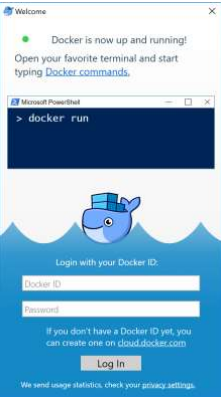
\includegraphics[width=5cm]{./Imagenes/1d}
		\end{center}	
\textbf{}\\
\textbf{}\\

\textbf{}\\
\textbf{}\\
\textbf{}\\
\textbf{}\\
\textbf{}\\

Para instalar MongoDB primero tenemos que ejecutar el siguiente código.
\textbf{}\\
\textbf{}\\
\begin{center}
		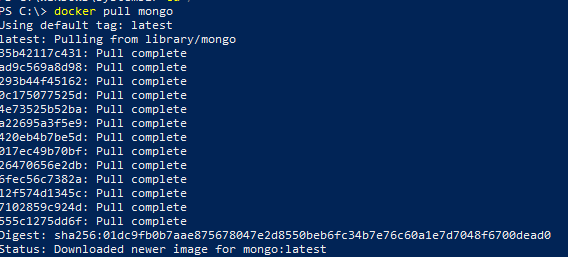
\includegraphics[width=9cm]{./Imagenes/2d}
		\end{center}	
\textbf{}\\
\textbf{}\\
Verificar que el contenedor se esté ejecutando correctamente mediante el comando:

\begin{center}
		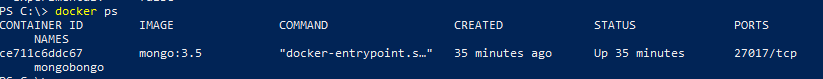
\includegraphics[width=9cm]{./Imagenes/3d}
		\end{center}	
\textbf{}\\
\textbf{}\\
Proceder a verificar la imagen con el siguiente comando:

\begin{center}
		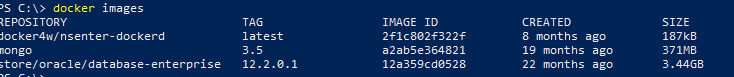
\includegraphics[width=9cm]{./Imagenes/4d}
		\end{center}	
\textbf{}\\
\textbf{}\\
Seguidamente ejecutar el comando. Como respuesta
se visualizará un ID que corresponde al contenedor:

\textbf{}\\
\textbf{}\\
\begin{center}
		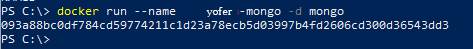
\includegraphics[width=9cm]{./Imagenes/5d}
		\end{center}	
\textbf{}\\
Para conectar a nuestro localhost
\textbf{}\\
\textbf{}\\
\begin{center}
		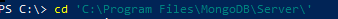
\includegraphics[width=9cm]{./Imagenes/6d}
		\end{center}	
\textbf{}\\
\textbf{}\\
Para exponer ese puerto para nuestro que podamos
acceder al contenedor
\textbf{}\\
\textbf{}\\
\begin{center}
		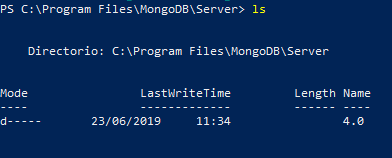
\includegraphics[width=9cm]{./Imagenes/7d}
		\end{center}	
\textbf{}\\
\textbf{}\\
MongoDB está preparado para escalar fácilmente
de manera horizontal
\textbf{}\\
\textbf{}\\
\begin{center}
		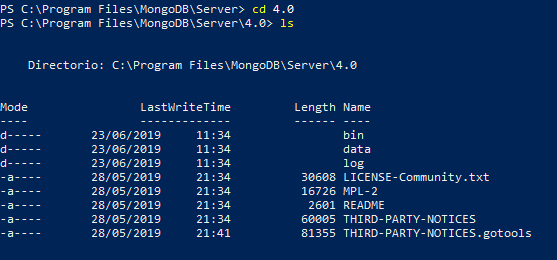
\includegraphics[width=9cm]{./Imagenes/8d}
		\end{center}	
\textbf{}\\
\textbf{}\\
En PowerShell ejecutar el siguiente comando, Verificar la eliminación del contenedor con ejecutando
\textbf{}\\
\textbf{}\\
\begin{center}
		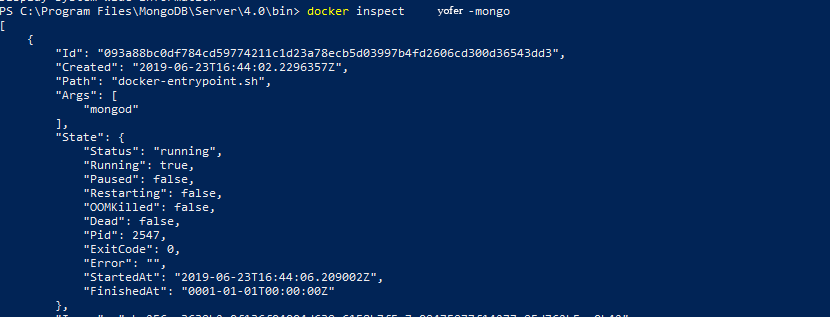
\includegraphics[width=9cm]{./Imagenes/9d}
		\end{center}	
\textbf{}\\
\textbf{}\\

Seguidamente ejecutar el comando: Como respuesta
se visualizará un ID que corresponde al contenedor
\textbf{}\\
\textbf{}\\
\begin{center}
		
\includegraphics[width=9cm]{./Imagenes/10d}
		\end{center}	
\textbf{}\\
\textbf{}\\

Para conectar a nuestro localhost
\textbf{}\\
\textbf{}\\
\begin{center}
		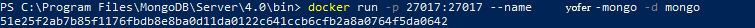
\includegraphics[width=9cm]{./Imagenes/11d}
		\end{center}	
\textbf{}\\
\textbf{}\\

conexión de Mongo, instancia de Mongo Corriendo
dentro de este contenedor Docker
\textbf{}\\
\textbf{}\\
\begin{center}
		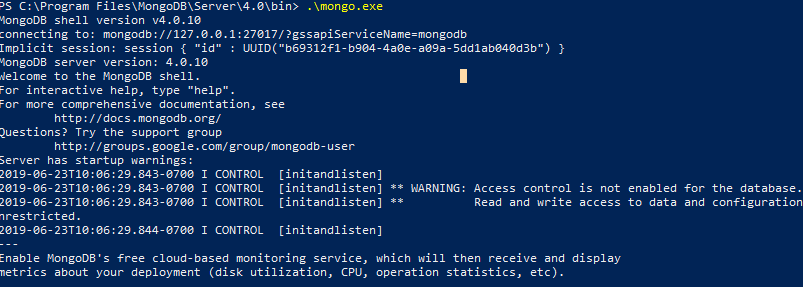
\includegraphics[width=9cm]{./Imagenes/12d}
		\end{center}	
\textbf{}\\
\textbf{}\\
\textbf{}\\
\textbf{}\\
\begin{center}
		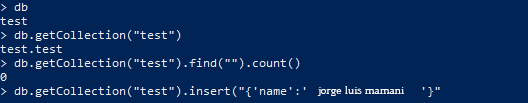
\includegraphics[width=9cm]{./Imagenes/13d}
		\end{center}	
\textbf{}\\
\textbf{}\\

\subsection{Inserción de datos y Consulta de datos (en una base de datos NOSQL)}
\begin{center}
		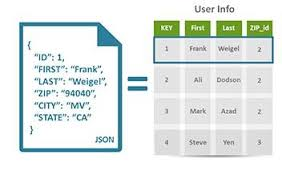
\includegraphics[width=9cm]{./Imagenes/6}
		\end{center}	
\textbf{}\\
Existen varias diferencias con respecto a cómo los distintos tipos de bases de datos permiten a los usuarios / aplicaciones realizar consultas. Desde las consultas más básicas por clave primaria, como por ejemplo, los almacenes clave – valor, pasando por otros que ofrecen un acceso a la información algo más complejo. En este terreno se encontrarían las bases de datos documentales.
\begin{center}
		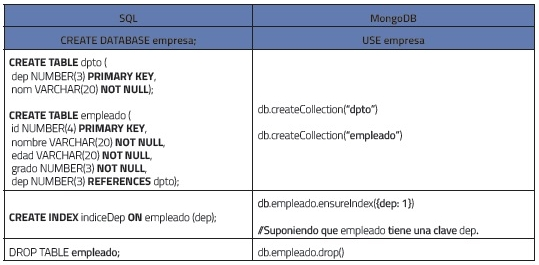
\includegraphics[width=9cm]{./Imagenes/1}
		\end{center}	
\textbf{}\\
En general, la flexibilidad y la riqueza de las querys no son demasiado elevadas, puesto que lo que se prima por encima de las consultas es el rendimiento y la escalabilidad, por lo que es habitual que se delegue a la aplicación el implementar opciones más avanzadas en este terreno.
\textbf{}\\
Un método de consulta llamado Companion SQL database consiste en tener una base de datos auxiliar (que puede ser una base de datos SQL o una TextDB) de forma que se utilice esta secundaria para almacenar ciertos metadatos importantes para realizar la búsqueda, y se empleen para facilitar la búsqueda posterior en el contenedor NoSQL.
\begin{center}
		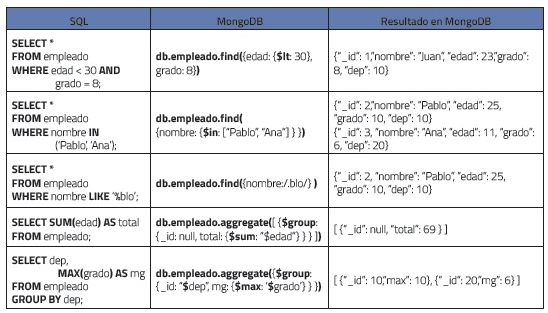
\includegraphics[width=9cm]{./Imagenes/2}
		\end{center}	
\textbf{}\\
Búsqueda local dispersa. Otra forma de realizar consultas consiste en, puesto que se tiene el conjunto de datos repartido entre los distintos servidores, repartir de igual modo la consulta, de forma que cada servidor ejecute localmente cada consulta y reenvíe los
resultados a un nodo maestro, que sería el encargado de juntar todos los resultados y presentárselos a la aplicación.
\textbf{}\\
Arboles B+ Distribuidos.
\textbf{}\\
Una forma eficiente de acelerar las búsquedas consiste en mantener un árbol B+ que forme un índice de entradas a la base de datos NoSQL (Aquilera, Golab and Shah 2008).
\textbf{}\\
El procedimiento consistiría en sacar los valores hash de los atributos que nos interese indexar, y construir con ellos el árbol B+. Cuando se quiera realizar una consulta, se comenzará desde la raíz y se irá descendiendo en orden hasta llegar a la hoja correspondiente, que nos dará la entrada concreta donde se encuentra el registro que se está buscando.
\begin{center}
		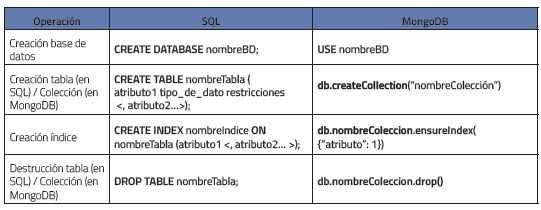
\includegraphics[width=9cm]{./Imagenes/3}
		\end{center}	
\textbf{}\\
Al tratarse de un árbol B+, se debe tener en cuenta las particularidades de este tipo de estructura de datos a la hora de realizar los mantenimientos necesarios, las inserciones y borrados que puedan hacer redimensiones en el árbol, etc.


\textbf{}\\
\subsection{Comparacion de distintos tipos de base de datos NoSQL}
\textbf{}\\Dependiendo de la forma en la que almacenen la información, nos podemos encontrar varios tipos
distintos de bases de datos NoSQL. Veamos los tipos más utilizados.
 \begin{itemize}
		\item Bases de datos clave – valor
                     \item Bases de datos documentales
		\item Bases de datos en grafo
		\item Bases de datos orientadas a objetos
	           \end{itemize}
\begin{center}
		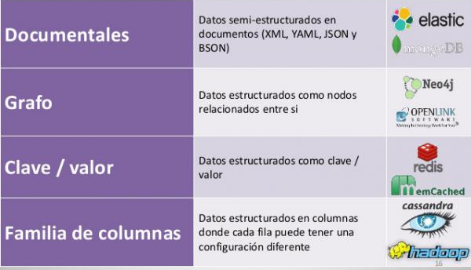
\includegraphics[width=9cm]{./Imagenes/7}
		\end{center}	
\textbf{}\\
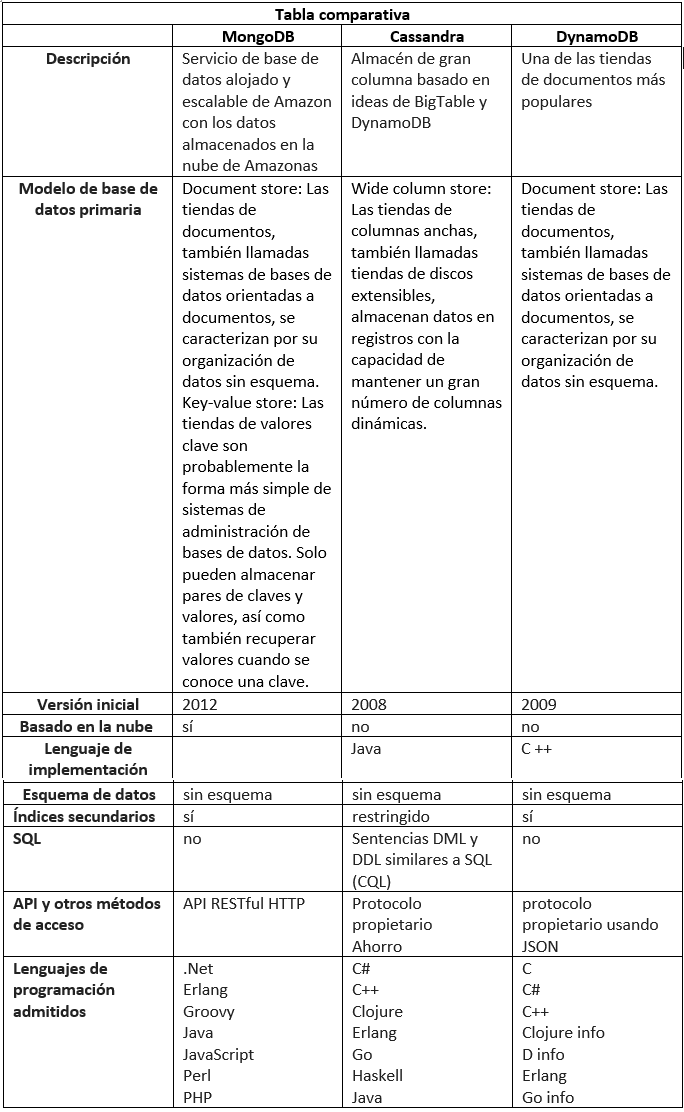
\includegraphics[scale=0.7]{Imagenes/tabla1.png}
\textbf{}\\
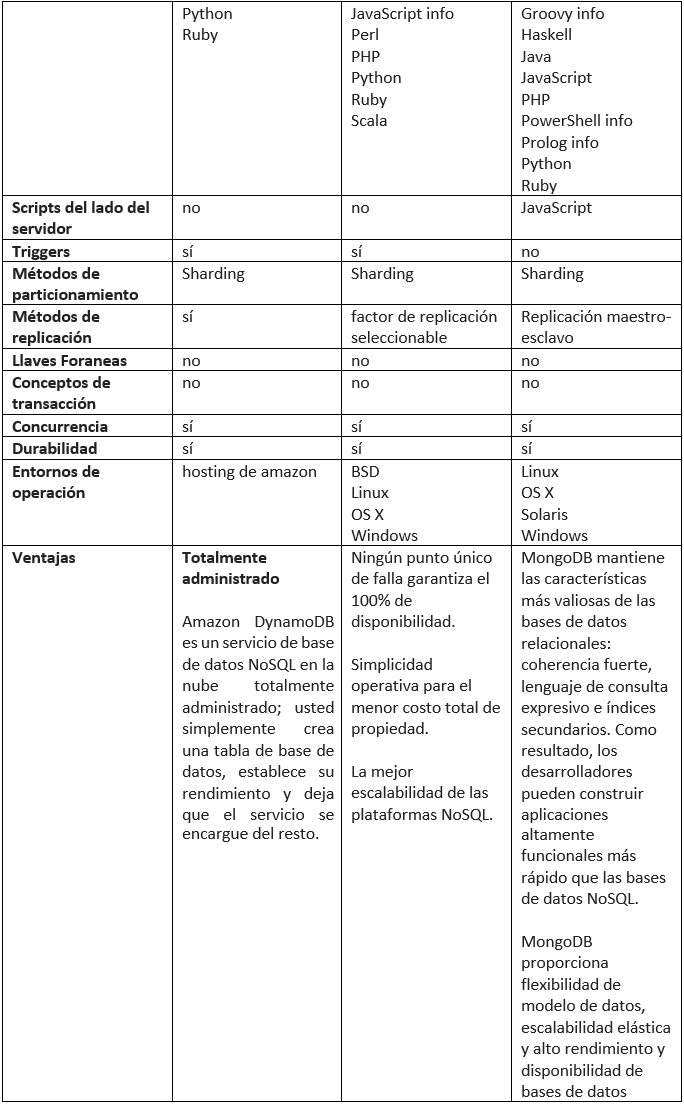
\includegraphics[scale=0.7]{Imagenes/tabla2.png}
\textbf{}\\
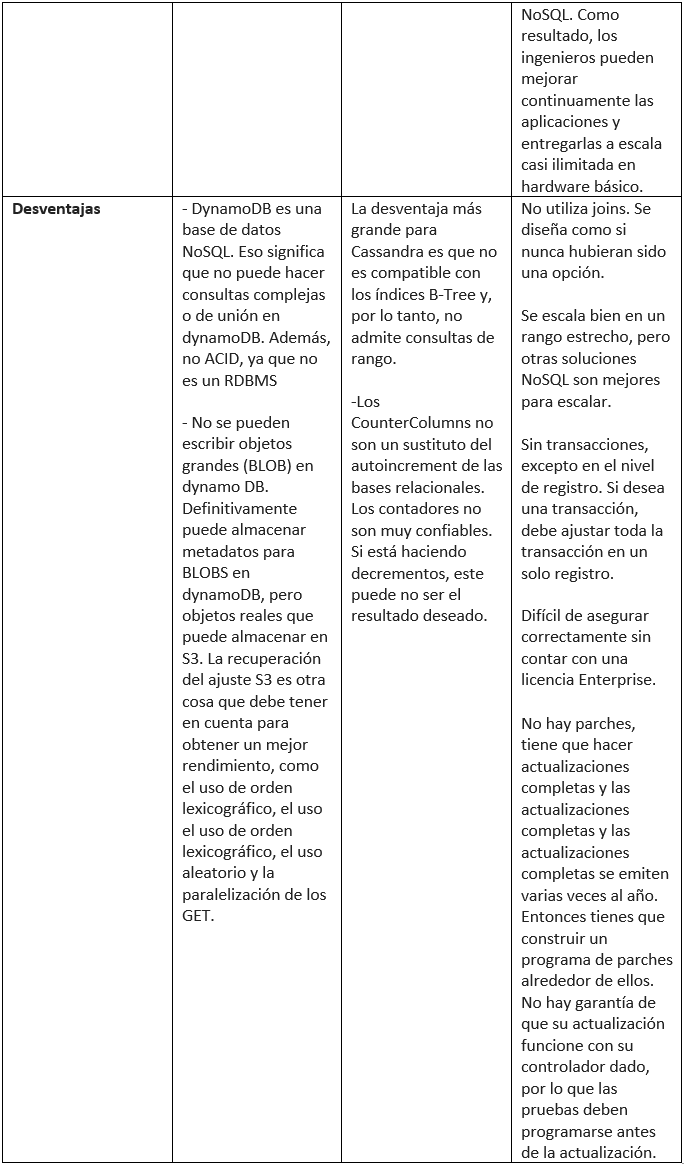
\includegraphics[scale=0.7]{Imagenes/tabla3.png}
\textbf{}\\


\textbf{CouchDB: }\\ CouchDB es catalogado muchas veces como una base de datos NoSQL, un término que se hizo cada vez más popular a finales de 2009 y principios de 2010. Si bien este término es una caracterización más bien genérica de una base de datos, o almacén de datos, sí define claramente un descanso de SQL tradicional bases de datos. Una base de datos CouchDB carece de un esquema o estructuras de datos pre-definidos rígidos tales como tablas. \textbf{}\\
Los datos almacenados en CouchDB es un documento (s) JSON. La estructura de los datos, o documento(s), puede cambiar dinámicamente para adaptarse a las necesidades cambiantes. 
CouchDB es una base de datos que abarca por completo la web. Almacene sus datos con documentos JSON. Tenga acceso a sus documentos y consultar sus índices con su navegador web, a través de HTTP.Índice, combinar y transformar sus documentos con JavaScript. CouchDB funciona bien con la web moderna y aplicaciones móviles. Usted puede incluso servir aplicaciones web directamente de CouchDB. Y usted puede distribuir sus datos o sus aplicaciones, de manera eficiente mediante la replicación incremental de los CouchDB. CouchDB soporta configuraciones maestro-maestro con detección automática de conflictos. \textbf{}\\
CouchDB viene con una serie de características, como la transformación de documentos sobre la marcha y notificaciones de cambio en tiempo real, que hace que el desarrollo de aplicaciones web una brisa. Incluso viene con un fácil utilizar la consola de administración web.\textbf{}\\
\textbf{}\\
 \textbf{Las principales características son las siguientes:}\\
\textbf{}\\
\textbf{•	Almacenamiento de documentos:}\\ Almacena los datos como documentos esto es, uno o más pares campo/valor expresados en JSON. Los valores de los campos pueden ser datos simples como cadenas de caracteres, números o fechas. Pero también se pueden usar listas ordenadas y vectores asociativos. Todos los documentos en una base de datos CouchDB tienen un identificador único y no requieren un esquema determinado.
\textbf{}\\
\textbf{}\\
\textbf{•	Vistas e índices Map/Reduce:}\\
 Los datos almacenados se estructuran por medio de vistas. En CouchDB, cada vista se construye por medio de una función JavaScript que actúa como la mitad Map de una operación map/reduce. La función recibe un documento y lo transforma en un único valor, retornándolo. CouchDB puede indexar vistas y mantener actualizados esos índices a medida que se agregan, eliminan o actualizan documentos.
\textbf{}\\
\textbf{•	Arquitectura distribuida con replicación: }\\
Se diseñó con teniendo en mente la replicación bidireccional (o sincronización) y la operación off-line. Eso significa que múltiples réplicas pueden tener cada una sus propias copias de los mismos datos, modificarlas y luego sincronizar esos cambios en un momento posterior.
\textbf{}\\
\textbf{}\\
\textbf{•	Interfaz REST:}\\
 Todos los ítems tienen una URI única que queda expuesta vía HTTP. REST usa los métodos HTTP POST, GET, PUT y DELETE para las cuatro operaciones básicas CRUD (Create, Read, Update, Delete) con todos los recursos.
\textbf{}\\
\textbf{}\\
\textbf{•	Consistencia Eventual:}\\
 Garantiza consistencia eventual para poder ofrecer tanto disponibilidad como tolerancia a las particiones.
\textbf{}\\
\textbf{}\\
\textbf{•	Hecha para operar offline:}\\
 Puede replicar datos a dispositivos (como smartphones) que pueden quedar offline y manejar automáticamente la sincronización de los datos cuando el dispositivo vuelve a estar en línea.


\textbf{}\\
\textbf{}\\
\textbf{}\\
\textbf{}\\

\textbf{Neo4j:}\\
 Es una base de datos orientada a grafos escrita en Java, es decir la información se almacena de forma relacionada formando un grafo dirigido entre los nodos y las relaciones entre ellos. Se integra perfectamente con múltiples lenguajes como Java, PHP, Ruby, .Net,  Python, Node, Scala, etc. La base de datos está embebida en un servidor Jetty. Está especialmente indicada para modelar redes sociales y sistemas de recomendación.\textbf{}\\
Se distribuye en dos versiones: la community edition (open source) y la Enterprise edition. Para hacer pruebas de concepto nos basta con la community edition pero si quieres sacarle todo el partido a Neo4j la opción enterprise es la más recomendable ya que permite ponerla en cluster, monitorización, backups en caliente y un sistema de cache de alto rendimiento, además de soporte de sus creadores.\textbf{}\\
Otra de las ventajas que tiene Neo4j es que se pueden efectuar las consultas directamente a través de un API Rest lo que hace especialmente interesante su integración con aplicaciones web.
\textbf{}\\
\textbf{Principales características de neo4j:}\\
\textbf{}\\
•	Alto desempeño y alta disponibilidad (Escalamiento de lectura) Soporte sólido y real para transacciones ACID.
\textbf{}\\
•	Escalable: 32 miles de millones de Nodos, 32 miles de millones de Relaciones, 64 miles de millones de Propiedades.
\textbf{}\\
•	Servidor con una API REST o usable como una biblioteca Java.


\textbf{}\\
\textbf{}\\
\textbf{}\\
\textbf{}\\
\textbf{}\\
\textbf{}\\
\textbf{}\\
\textbf{}\\
\textbf{}\\
\textbf{}\\
\textbf{}\\
\textbf{}\\
\textbf{}\\
\textbf{}\\
\textbf{}\\
\textbf{}\\
\textbf{}\\
\textbf{}\\

\section{Resultados}
\textbf{Comparaciones de 2 Bases de Datos NoSQL}\\
\subsection{Grafos}


\textbf{}\\En este caso usaremos Neo4j la cual es un base de datos NoSql, procedemos a descargar y a crear un nuevo proyecto.
\begin{center}
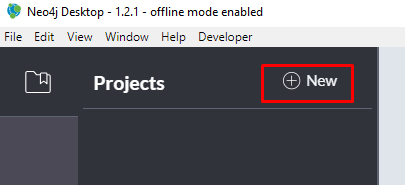
\includegraphics[scale=0.7]{Imagenes/neo4j}
\end{center}	
\textbf{}\\
\textbf{}\\Le damos un nombre a nuestro nodo y procedemos a iniciarlo.
\begin{center}
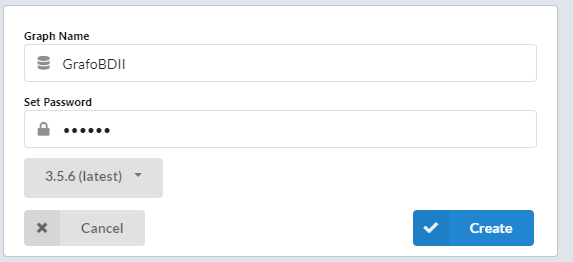
\includegraphics[scale=0.7]{Imagenes/neo4j2}
\begin{center}
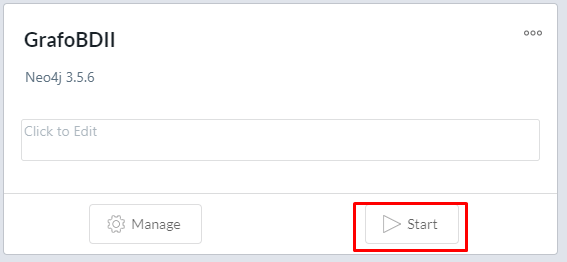
\includegraphics[scale=0.7]{Imagenes/neo4j3}
\end{center}	
\end{center}	
\textbf{}\\
\textbf{}\\Crearemos el siguiente nodo:
\begin{center}
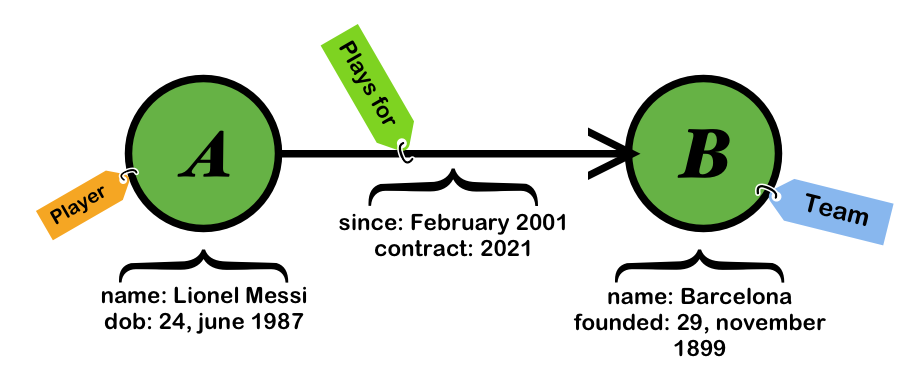
\includegraphics[scale=0.4]{Imagenes/neo4jn}
\end{center}	

\begin{center}
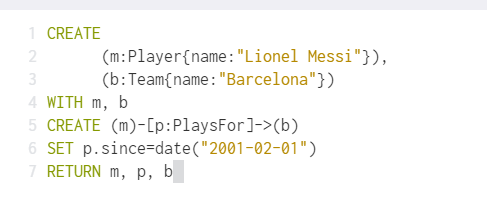
\includegraphics[scale=0.7]{Imagenes/neo4j5}
\end{center}	
\textbf{}\\ Y el resultado sera el siguiente:
\begin{center}
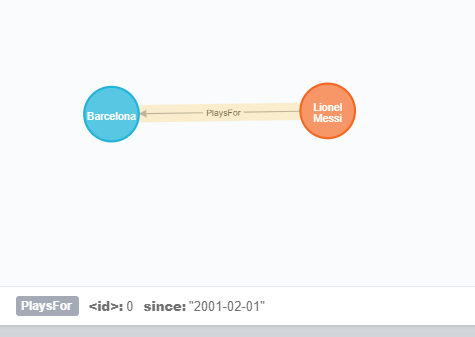
\includegraphics[scale=0.7]{Imagenes/neo4j7}
\end{center}	

\textbf{}\\ Ahora haremos un ejemplo mas complejo, creamos una red de amigos:

\begin{center}
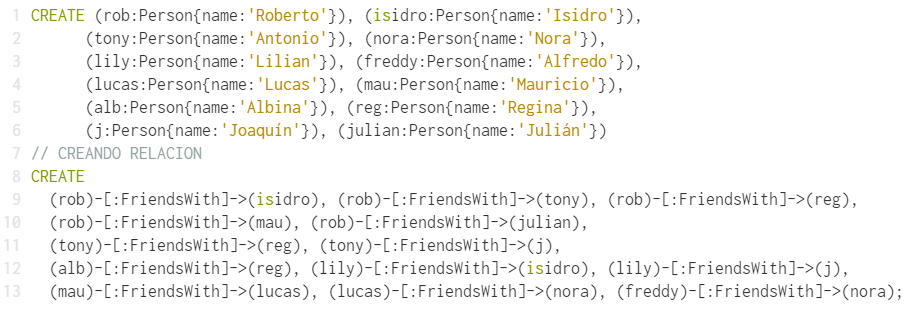
\includegraphics[scale=0.7]{Imagenes/neo4j6}
\end{center}	

\begin{center}
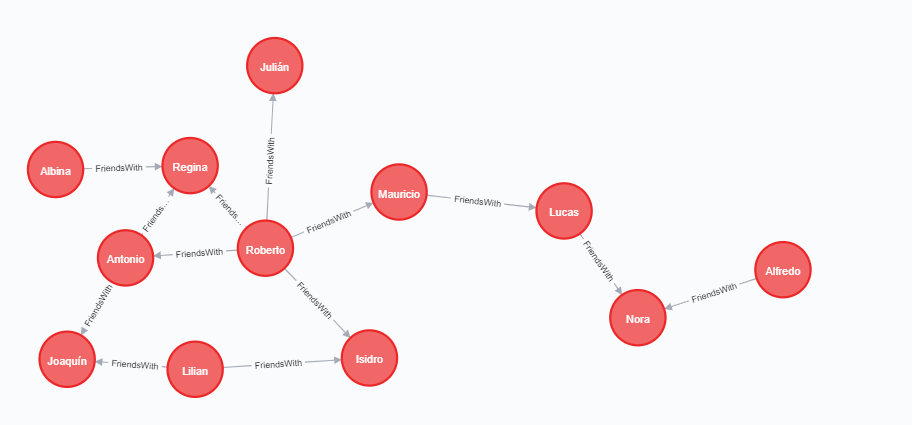
\includegraphics[scale=0.7]{Imagenes/neo4j8}
\end{center}	

\textbf{}\\
\textbf{}\\ Ahora averigüemos quiénes son amigos de Lucas :

\begin{center}
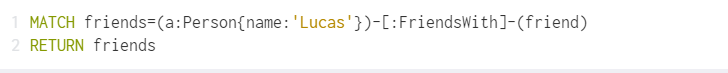
\includegraphics[scale=0.7]{Imagenes/neo4j9}
\end{center}	

\textbf{}\\Si queremos buscar los amigos de los amigos de Lucas seria con la siguiente consulta:

\begin{center}
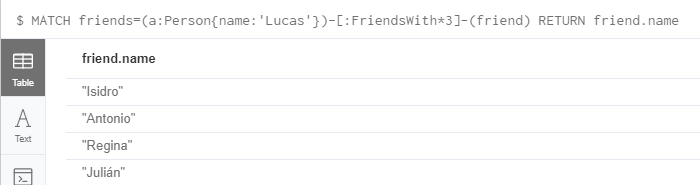
\includegraphics[scale=0.7]{Imagenes/neo4j10}
\end{center}	
\textbf{}\\ Esto haciendolo desde SQL seria muy dificil y tedioso pero aca lo hacemos de una manera muy facil.
\textbf{}\\ Finalmente podemos buscar el camino mas corto entre Joaquin y Lucas:

\begin{center}
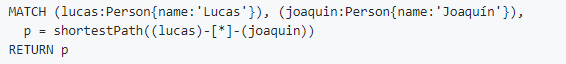
\includegraphics[scale=0.7]{Imagenes/neo4j12}
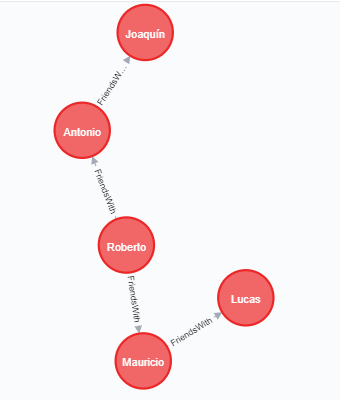
\includegraphics[scale=0.7]{Imagenes/neo4j11}
\end{center}	



\subsection{Base de datos Documental}

\textbf{}\\Una base de datos documental, también llamada una base de datos orientada a documentos u tienda de documentos, es un subconjunto de un tipo de base de datos NoSQL.
Algunos almacenes de documentos también pueden ser bases de datos de valores clave. Una base de datos de documentos se utiliza para almacenar, recuperar y administrar datos semiestructurados.
A diferencia de las bases de datos relacionales tradicionales, el modelo de datos en una base de datos de documentos no está estructurado en un formato de tabla de filas y columnas.
El esquema puede variar, proporcionando mucha más flexibilidad para el modelado de datos que las bases de datos relacionales.
Las bases de datos documental almacena cada registro y sus datos asociados en un solo documento. Cada documento contiene datos semiestructurados que pueden ser consultados con el uso de varias herramientas de consulta y análisis del DBMS.



\textbf{Funcionamiento}\\
Una base de datos de documentos utiliza documentos como la estructura para almacenamiento y consultas. En este caso, el término "documento" puede referirse a un documento de texto, pero comúnmente es un archivo de XML o JSON. En lugar de columnas con nombres y tipos de datos que se utilizan en una base de datos relacional, un documento contiene una descripción del tipo de datos y el valor de esa descripción.

\textbf{Ejemplo de Base de Datos Documental en XML}\\
\begin{center}
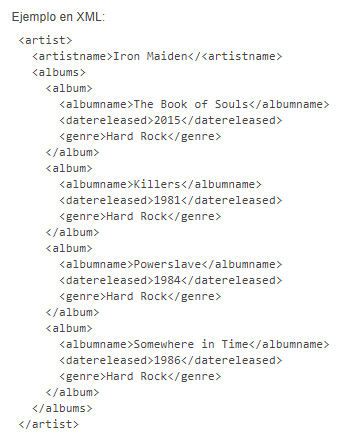
\includegraphics[scale=0.7]{Imagenes/EjemploDocumental.png}
\end{center}	

\textbf{Ejemplo de Base de Datos Documental en Json}\\
\begin{center}
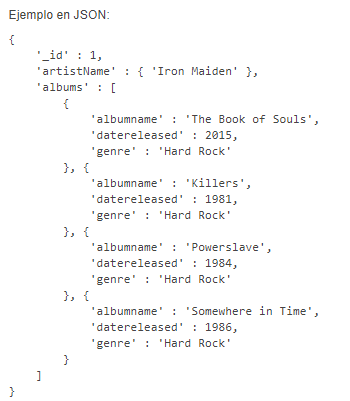
\includegraphics[scale=0.7]{Imagenes/EjemploDocumentalJson.png}
\end{center}

\textbf{Beneficios}\\
Las tiendas de documentos ofrecen importantes ventajas cuando se requieren características específicas, que incluyen:
Modelado flexible de datos: a medida que las aplicaciones web, móviles, sociales e IoT cambian la naturaleza de los modelos de datos de aplicaciones, las bases de datos de documentos eliminan la necesidad de forzar modelos de datos relacionales para admitir nuevos tipos de modelos de datos de aplicaciones.
Rendimiento de escritura rápido: a diferencia de las bases de datos relacionales tradicionales, algunas bases de datos de documentos priorizan la disponibilidad de escritura sobre la estricta consistencia de los datos. Esto garantiza que las escrituras siempre serán rápidas, incluso si una falla en una parte del hardware o de la red da como resultado un pequeño retraso en la replicación de datos y la coherencia en todo el entorno.
Rendimiento rápido de consultas: muchas bases de datos de documentos tienen potentes motores de búsqueda y funciones de indexación que proporcionan capacidades de consulta rápidas y eficientes.


\subsection{Base de Datos Valor - Clave}
\textbf{}\\Una base de datos de valores-clave (también conocida como almacén de valores-clave y base de datos key-value) es un tipo de base de datos NoSQL que utiliza un método simple de clave / valor para almacenar datos.
La parte clave-valor se refiere al hecho de que la base de datos almacena datos como una colección de pares clave / valor. Este es un método simple de almacenar datos, y se sabe que escala bien.
El par clave-valor es un concepto bien establecido en muchos lenguajes de programación. Los lenguajes de programación normalmente se refieren a una clave-valor como una matriz asociativa o estructura de datos. Un valor-clave también se conoce comúnmente como diccionario o hash.
Un store de valores-clave o una base de datos de valores-clave es una base de datos simple que usa un arreglo asociativo (piensa en un mapa o diccionario) como el modelo de datos fundamental donde cada clave está asociada con un solo valor en una colección. Esta relación se conoce como un par clave-valor.

\textbf{Ejemplos de base de datos clave-valor}\\
A continuación hay ejemplos de tiendas de valores clave.
Estos son ejemplos simples, pero el objetivo es proporcionar una idea de cómo funciona una base de datos clave-valor.
\begin{center}
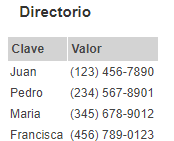
\includegraphics[scale=0.7]{Imagenes/ClaveValor.png}
\end{center}
\textbf{¿Qué tipo de datos se pueden almacenar en una base de datos clave-valor?}\\

\textbf{La clave}\\
La clave en un par clave-valor debe (o al menos, debería) ser única. Este es el identificador único que le permite acceder al valor asociado con esa clave.
En teoría, la clave podría ser cualquier cosa. Pero esto puede depender del DBMS. Un DBMS puede imponer limitaciones mientras que otro puede imponer ninguno.
En Redis, por ejemplo, el tamaño de clave máximo permitido es 512 MB. Puede usar cualquier secuencia binaria como clave, desde una secuencia de texto corta hasta el contenido de un archivo de imagen. Incluso la cadena vacía es una clave válida.
Sin embargo, por motivos de rendimiento, debe evitar tener una clave demasiado larga.
Pero una clave demasiado corta también puede causar problemas de legibilidad. En cualquier caso, la clave debe seguir una convención convenida para mantener las cosas consistentes.

\textbf{El valor}\\

El valor en un almacén de clave-valor puede ser cualquier cosa, como texto (largo o corto), un número, código de marcado como HTML, código de programación como PHP, una imagen, etc.
El valor también podría ser una lista, o incluso otro par clave-valor encapsulado en un objeto.
Algunos DBMS de almacenamiento de claves le permiten especificar un tipo de datos para el valor. Por ejemplo, puede especificar que el valor sea un entero. Otros DBMS no proporcionan esta funcionalidad y, por lo tanto, el valor podría ser de cualquier tipo.

\textbf{¿Para qué se puede usar una base de datos de valores-clave?}\\

Las bases de datos de valores clave se pueden aplicar a muchos escenarios. Por ejemplo, las tiendas de valores clave pueden ser útiles para almacenar cosas como las siguientes.









\textbf{}\\
\textbf{}\\
%----------------------------------------------------------------------------------------
%	REFERENCE LIST
%----------------------------------------------------------------------------------------

\begin{thebibliography}{99} % Bibliography - this is intentionally simple in this template



\newblock 
1. http://revistatelematica.cujae.edu.cu/
index.php/tele/article/view/23/21
 \break
\newblock 
2. https://programarfacil.com/blog/
que-es-un-orm/
\break
\newblock 
3. https://www.beeva.com/beeva-view/tecnologia/mas-alla-de-la-virtualizacion-contenedores/
\break
\newblock
4. https://searchdatacenter.techtarget.com/
es/definicion/virtualizacion-basada-en-contenedores-virtualizacion-a-nivel-de-sistema-operativo
\break
\newblock
5. https://www.incibe-cert.es/blog/asegurando-virtualizacion-tus-sistemas-control
\break
\newblock
6. http://www.datakeeper.es/?p=716
\break
\newblock
7.https://sigmodrecord.org/publications/sigmodRecord/1012/pdfs/04.surveys.cattell.pdf
\break
\newblock
8.https://ieeexplore.ieee.org/abstract/document/6625441
\break
\newblock
9.-http://nosql-database.org/
\break
\newblock
10.-https://www.oracle.com/technetwork/es/articles/datawarehouse/oracle12c-docker-win10-4485487-esa.html
\break
\newblock {\em }
 
\end{thebibliography}



%----------------------------------------------------------------------------------------
\end{itemize}
\end{flushright}
\end{document}

